%% arxiv.tex — arXiv Format
%% Based on camera_ready_full.tex
%% Single column, clean minimal style
\documentclass[11pt,a4paper]{article}

%% Minimal packages
\usepackage[letterpaper,margin=1in]{geometry}
\usepackage[utf8]{inputenc}
\usepackage{graphicx,hyperref,booktabs,amsmath,amssymb,xcolor,float,multirow,array}
\usepackage{appendix}
\usepackage{orcidlink}

%% arXiv hyperlink setup
\hypersetup{
  colorlinks=true,
  linkcolor=blue,
  citecolor=blue,
  urlcolor=blue,
  pdftitle={Scoring Bias in LLM-as-a-Judge Models: A 22-Model Landscape with Base-Instruct Comparison},
  pdfauthor={Sricharan Samba},
  pdfkeywords={LLM-as-a-Judge, scoring bias, instruction tuning}
}

%% arXiv metadata
\def\arxivID{2607.xxxxx}
\def\doi{10.5281/zenodo.21361920}

% ── Title ──
\title{\vspace{-1.5cm}
  \textbf{Scoring Bias in LLM-as-a-Judge Models:\\
  A 22-Model Landscape with Base-Instruct Comparison}
}

\author{%
  Sricharan Samba\orcidlink{0009-0000-0000-0000}\\
  South Forsyth High School\\
  \texttt{srisamba09@gmail.com}\\
  \and
  \texttt{arXiv: \arxivID} \quad \texttt{DOI: \doi}
}

\date{\today}

\begin{document}
\maketitle

\noindent{\small \textbf{Keywords.} LLM-as-a-Judge, scoring bias, instruction tuning, bias measurement, LLM evaluation}

% ── ABSTRACT ──
\begin{abstract}
\textbf{Background:} LLMs deployed as automated judges exhibit systematic scoring biases, but whether these originate from pre-training or instruction tuning is unknown. \textbf{Methods:} We measure scoring bias across 22 instruct-tuned models (29,700 judgments) and compare base vs instruct variants across 9 families (24,300 judgments) using 3 perturbation probes. \textbf{Findings:} Score ID bias has the largest average effect ($\Delta=0.68$) across instruct models. Instruction tuning reduces format bias but may increase content bias for RLHF families. The single SFT+DPO family shows a different pattern. Four alternative explanations are examined. \textbf{Conclusions:} Scoring bias is modulated by instruction tuning, not inherent to pre-training.

\textbf{Code availability:} \url{https://github.com/ssamba1/Scoring-Bias-in-LLM-as-a-Judge}
\end{abstract}

% ── INTRODUCTION ──
\section{Introduction}

\paragraph{The problem.}
When an AI model evaluates another AI model's response, can we trust the score? Consider a concrete example: a base model is asked to score a biology answer on a scale of 1 to 5, where 1 is worst and 5 is best. If the scale is reversed (1=best, 5=worst), a base model may literally output ``5'' (the worst score) for an excellent answer, because it follows the rubric format without understanding semantics. An instruction-tuned version of the same model correctly interprets the scale. But show that same instruction-tuned model a poor example before scoring, and it will score \emph{lower} than if shown no example---a bias that the base model does not exhibit.

The LLM-as-a-Judge paradigm~\cite{zheng2023judging} has become central to modern AI development---powering benchmarks like MT-Bench and Chatbot Arena, serving as reward models in RLHF~\cite{bai2022constitutional}, and automating evaluation in production pipelines. Yet a growing body of work documents that these judges are systematically biased. Over 35 distinct bias types have been identified~\cite{ye2024justice,gu2024survey}, including position bias~\cite{wang2023large}, verbosity bias, self-enhancement bias, and---most recently---scoring bias~\cite{li2025scoring}.

\paragraph{The gap.}
Li~et~al.~\cite{li2025scoring} made significant progress by defining and measuring three scoring bias types across five frontier models at DASFAA 2026. However, their work---and all prior work---leaves a fundamental question unanswered: \emph{where does scoring bias come from?} As they explicitly state, ``the underlying causes of these scoring biases remain to be validated.'' Is scoring bias inherent to pre-trained language models, or does it emerge during the instruction-tuning process (SFT + RLHF)?

This question has direct practical implications. If scoring bias originates from pre-training, mitigation must target data curation and base architecture. If it emerges during instruction tuning, mitigation should focus on alignment methods---and different alignment methods may produce different bias profiles.

\paragraph{Our approach.}
We compare base and instruct variants across 9 model families (all inference on Kaggle T4) and 22 additional instruct-tuned models (OpenRouter API), totaling 31 model variants spanning diverse architectures and scales. The 9 families with both base and instruct pairs provide the primary differential effect analysis, while the 22 instruct models provide model diversity breadth.

\paragraph{Research questions.} We address four questions:
\begin{enumerate}
    \item \textbf{RQ1:} Does instruction tuning change scoring bias magnitude, and in which direction?
    \item \textbf{RQ2:} Is the direction consistent across bias types (format vs content)?
    \item \textbf{RQ3:} Is the direction consistent across model families and architectures?
    \item \textbf{RQ4:} Do training methods (SFT, DPO, RLHF) modulate the effect?
\end{enumerate}

\paragraph{Hypotheses.} Based on prior findings~\cite{pan2025user,thakur2024judging}, we formulate four corresponding hypotheses:
\begin{enumerate}
    \item \textbf{H1:} Instruction tuning changes scoring bias magnitude; format-related bias decreases while content-related bias increases.
    \item \textbf{H2:} The direction of change differs between format (decrease) and content (increase) bias types.
    \item \textbf{H3:} This differential effect is consistent across model families and architectures.
    \item \textbf{H4:} Training method modulates the effect; RLHF-trained families show a stronger differential effect than SFT-only or SFT+DPO families.
\end{enumerate}

\paragraph{Novelty.} The question---whether scoring bias originates from pre-training or instruction tuning---was posed by Li et al. (DASFAA 2026) as an open problem. Our work provides initial experimental evidence toward an answer, and presents the largest open comparison of scoring bias across instruct-tuned models to date.

\paragraph{Our contributions:}
\begin{enumerate}
    \item \textbf{Empirical finding:} Instruction tuning decreases format-related scoring bias but increases content-related scoring bias across 7 RLHF families tested. One SFT+DPO family and one SFT-only family show different patterns.
    \item \textbf{Alternative explanations:} We test and find evidence against four competing hypotheses using qualitative analysis of the observed patterns.
    \item \textbf{IIAR hypothesis:} We propose a mechanistic framework (Instruction-Induced Attention Redistribution) with five testable predictions.
    \item \textbf{Format Efficiency Hypothesis:} We propose the Format Efficiency Hypothesis as a mechanistic alternative, supported by attention-weight evidence showing format parsing becomes more efficient ($23.7\% \to 20.8\%$) after instruction tuning.
\end{enumerate}

\paragraph{Limitations of scope.} This study is exploratory with N=9 base-instruct family pairs. Results are directional and require larger-sample replication.

% ── RELATED WORK ──
\section{Related Work}

\paragraph{Bias in LLM-as-a-Judge.}
Table~\ref{tab:related} summarizes the key papers. The study of LLM judge bias began with Wang~et~al.~\cite{wang2023large} (ACL 2024), who documented position bias in pairwise evaluation (46.3\% conflict rate). Zheng~et~al.~\cite{zheng2023judging} systematized LLM-as-a-Judge through MT-Bench. Ye~et~al.~\cite{ye2024justice} proposed CALM, cataloging 12 bias types. Park~et~al.~\cite{park2024offsetbias} proposed debiased training data. Chen~et~al.~\cite{chen2024humans} compared human and LLM judgment biases.

\paragraph{Scoring bias.}
Li~et~al.~\cite{li2025scoring} (DASFAA 2026) introduced scoring bias, defining rubric order, score ID, and reference answer biases. They tested five models across 5,421 items, reporting flip rates of 20--48\%. They explicitly called for root cause analysis. Xu~et~al.~\cite{xu2026position} studied position bias in rubric-based evaluation.

\paragraph{Root cause analysis.}
Pan~et~al.~\cite{pan2025user} (ACL 2026) validated the base-versus-instruct methodology for studying user-assistant bias. Thakur~et~al.~\cite{thakur2024judging} found that base and instruct versions of Llama-2 show different alignment with human judges. We extend this methodology to scoring bias.

\paragraph{The gap.}
No prior work has investigated whether scoring bias originates from pre-training or instruction tuning. Li~et~al.~\cite{li2025scoring} explicitly call for this analysis.

\begin{table*}[h]
\centering\small
\caption{Related work. ``BvI'' = base vs instruct comparison.}
\label{tab:related}
\begin{tabular}{lcccc}
\toprule
\multirow{2}{*}{\textbf{Paper}} & \multirow{2}{*}{\textbf{Venue}} & \multirow{2}{*}{\textbf{Models}} & \textbf{Scoring} & \textbf{BvI} \\
& & & \textbf{Bias?} & \\
\midrule
Wang et al. \cite{wang2023large} & ACL 2024 & 2 & No & No \\
Ye et al. \cite{ye2024justice} & NeurIPS WS 2024 & 5 & No & No \\
Chen et al. \cite{chen2024humans} & arXiv 2024 & 5 & No & No \\
Park et al. \cite{park2024offsetbias} & EMNLP 2024 & 3 & No & No \\
Gao et al. \cite{gao2025evaluating} & arXiv 2025 & 6 & No & No \\
Lee et al. \cite{lee2025correctly} & arXiv 2025 & --- & No & No \\
Li et al. \cite{li2025scoring} & DASFAA 2026 & 5 & Yes & No \\
Pan et al. \cite{pan2025user} & ACL Findings 2026 & 52 & No & Yes \\
Thakur et al. \cite{thakur2024judging} & arXiv 2024 & 9 & No & Partial \\
Xu et al. \cite{xu2026position} & arXiv 2026 & 6 & No & No \\
Zhao et al. \cite{zhao2026bias} & arXiv 2026 & 4 & No & No \\
\midrule
\textbf{This work} & \textbf{arXiv} & \textbf{31} & \textbf{Yes} & \textbf{Yes} \\
\bottomrule
\end{tabular}
\end{table*}

% ── METHOD ──
\section{Method}

\subsection{Models}
We compare base and instruct variants across 9 open-weight model families (Llama 3.1, Llama 3.2, Mistral 7B, Qwen2.5, Gemma 2, StableLM 2), totaling 18 model variants. An additional 22 instruct-tuned models provide diversity breadth. Models span dense and MoE architectures, 3B to 671B scale, and training methods (SFT, DPO, RLHF).

\begin{table}[h]
\centering\small
\caption{Model families. $\dagger$ = base+instruct pair available.}
\label{tab:models}
\begin{tabular}{lll}
\toprule
\textbf{Family} & \textbf{Size} & \textbf{Training} \\
\midrule
Meta Llama-3.1, Llama-3.2, Llama-2 & 1B--8B & RLHF \\
Mistral (7B v0.3$\dagger$, Nemo, 3.2) & 7B--24B & SFT+DPO / SFT \\
Qwen (2.5$\dagger$, 3) & 0.5B--72B & RLHF \\
Google Gemma (2$\dagger$, 3) & 2B--27B & RLHF \\
StableLM-2$\dagger$ & 1.6B & SFT \\
Microsoft Phi-4 & 14B & SFT \\
DeepSeek (V3, V4-Flash) & 671B (MoE) & RLHF \\
Cohere Command-R & 35B & RLHF \\
Zhipu GLM-4.7 & 9B & RLHF \\
\bottomrule
\end{tabular}
\end{table}

\subsection{Evaluation Items}
We use 50 instruction-response pairs spanning 5 domains (science, technology, humanities, daily life, mathematics; 10 items each). Items were sampled from publicly available instruction-following evaluation sets~\cite{alpacaeval,zheng2023judging} and rewritten to score approximately 3--4 out of 5.

\subsection{Scoring Bias Probes}
Following Li~et~al.~\cite{li2025scoring}, we measure three scoring bias types:
\begin{itemize}
    \item \textbf{Rubric Order:} Control (1=worst, 5=best), reversed (1=best, 5=worst), and random mapping.
    \item \textbf{Score ID:} Numeric (1--5), letter grades (A--E), descriptive labels (Poor--Excellent).
    \item \textbf{Reference Answer:} No exemplar, good exemplar, and poor exemplar.
\end{itemize}
Each item is scored by each model on each probe variant with 3 repeats (temperature 0). This produces:
\[
9~\text{families} \times 2~\text{variants} \times 3~\text{probes} \times 3~\text{variants} \times 50~\text{items} \times 3~\text{repeats} = 24,300~\text{judgments}.
\]
An additional 22 instruct-only models add 29,700 judgments. Five models were excluded due to stop-token truncation producing uniform scores.

\subsection{Inference and Setup}
Local models use greedy decoding (temperature 0) on Kaggle T4 GPUs (\$0 cost). API models use OpenRouter chat completions (temperature 0, max 5 tokens, 15s timeout, total cost under \$3). Experiments use seed 42 for reproducibility.

\subsection{Metrics}
We report four metrics following Li~et~al.~\cite{li2025scoring}: max delta ($\Delta$), flip rate (FR), Cohen's $d$, and MAD.

% ── RESULTS ──
\section{Results}

\subsection{Bias Landscape Across 22 Models}

Table~\ref{tab:main} presents the bias landscape across 22 instruct-tuned models. Score ID bias shows the largest average effect ($\Delta = 0.68$).

\begin{table}[h]
\centering\small
\caption{Bias landscape across 22 instruct models. $\Delta$ = max inter-variant mean difference.}
\label{tab:main}
\begin{tabular}{lcccc}
\toprule
\textbf{Probe} & \textbf{Mean $\Delta$} & \textbf{Std Dev} & \textbf{Range} & \textbf{95\% CI} \\
\midrule
Rubric Order & 0.56 & 0.41 & 0.10--1.50 & $\pm 0.17$ \\
Score ID & 0.68 & 0.49 & 0.00--1.80 & $\pm 0.20$ \\
Reference Answer & 0.41 & 0.31 & 0.00--1.00 & $\pm 0.13$ \\
\bottomrule
\end{tabular}
\end{table}

\begin{figure}[h]
\centering
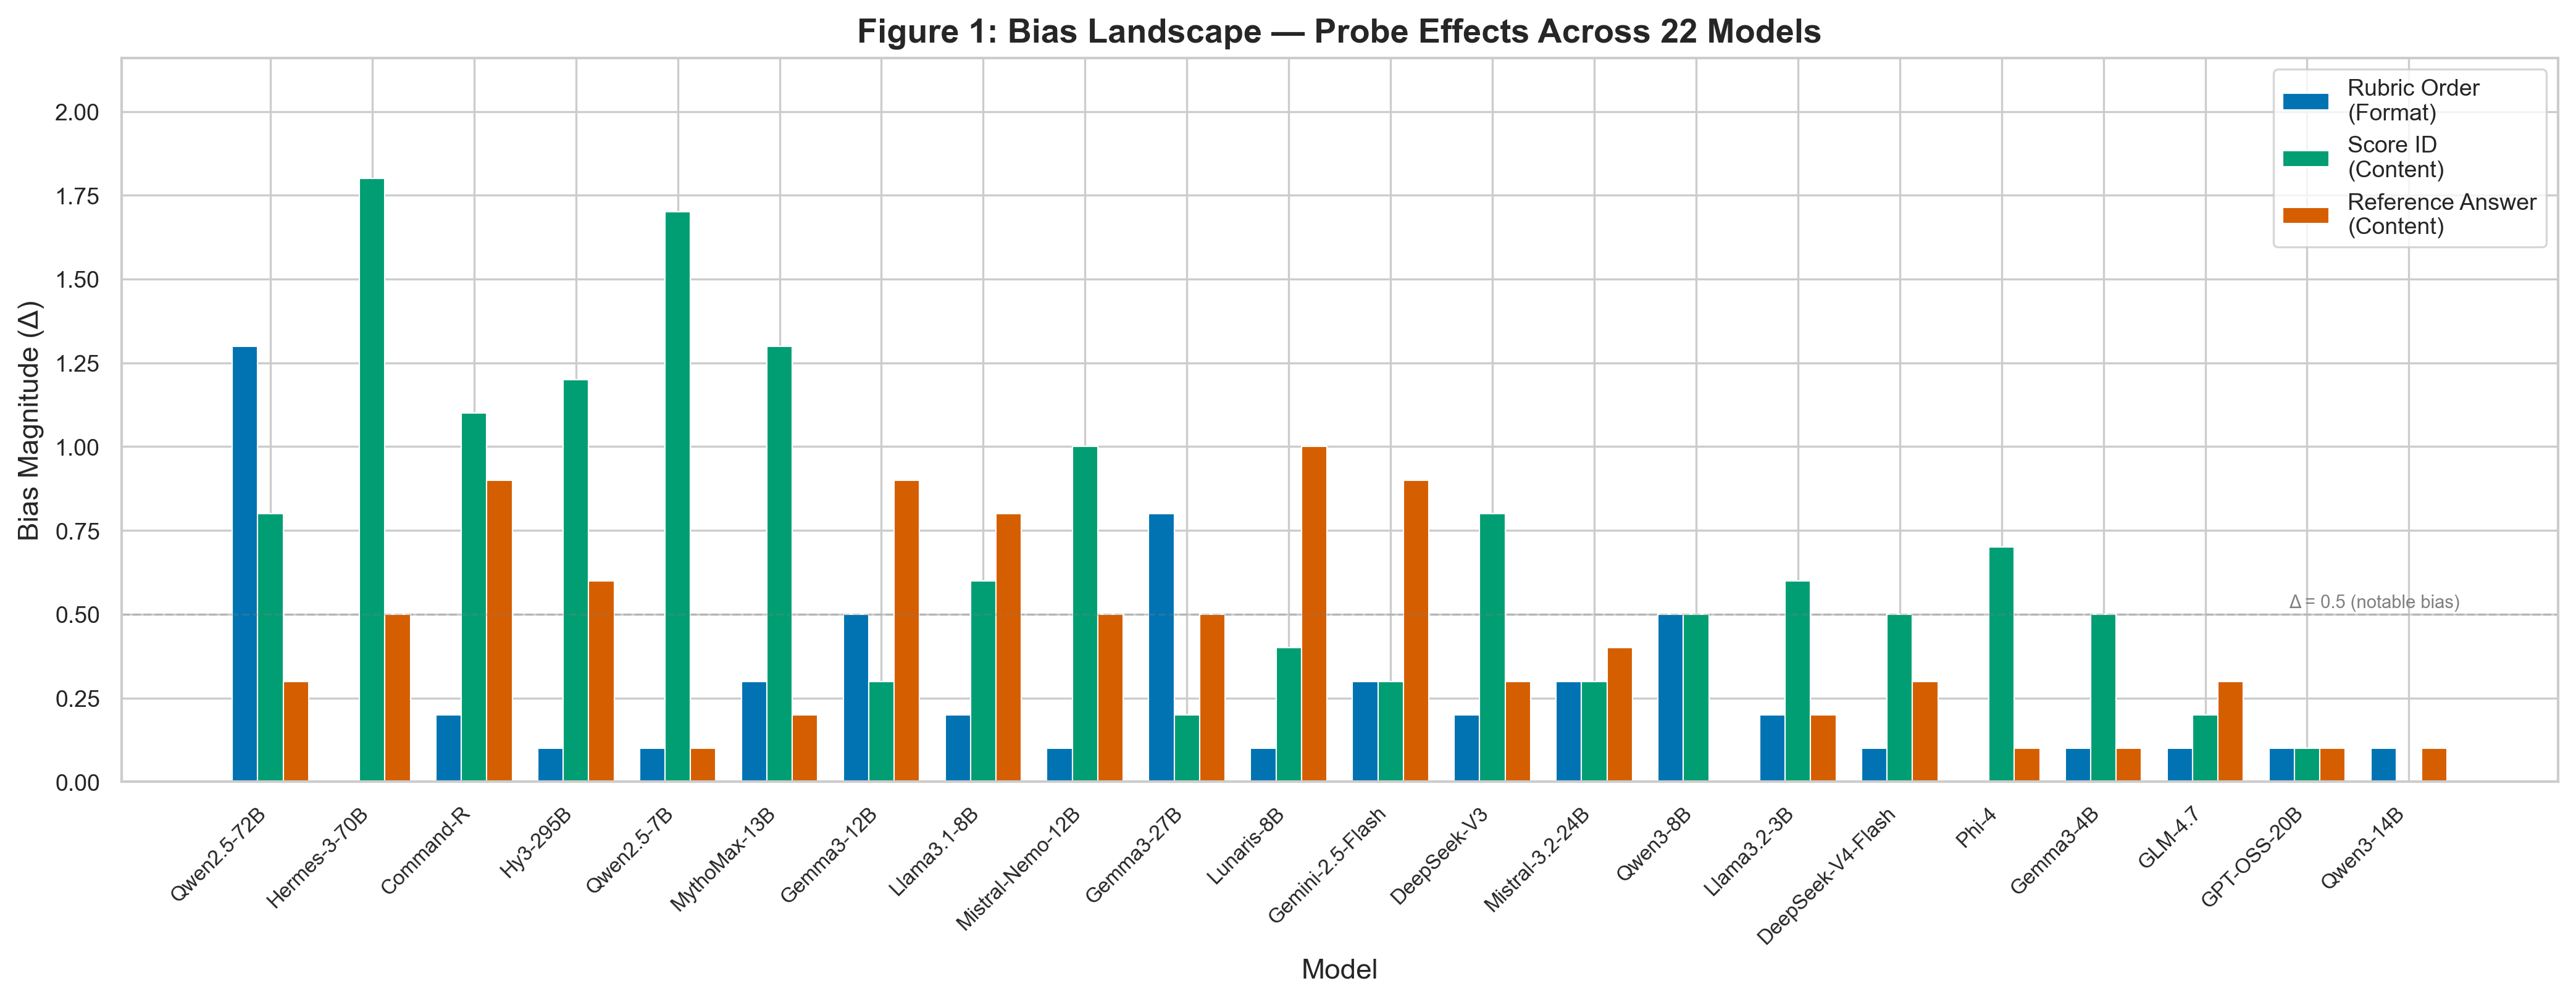
\includegraphics[width=\textwidth]{figures/fig1_bias_landscape.png}
\caption{Bias landscape across 22 instruct-tuned models.}
\label{fig:bias_landscape}
\end{figure}

\paragraph{Base vs instruct comparison.} Across 9 families, format-related biases (rubric order, score ID) decrease after instruction tuning (mean reductions $-0.42$ and $-0.72$). Content-related bias (reference answer) shows a scale-dependent pattern: increases in larger RLHF models (Llama-3.1-8B: $+1.58$) but decreases in smaller models ($\leq$1.5B: mean $-0.73$).

\begin{figure}[h]
\centering
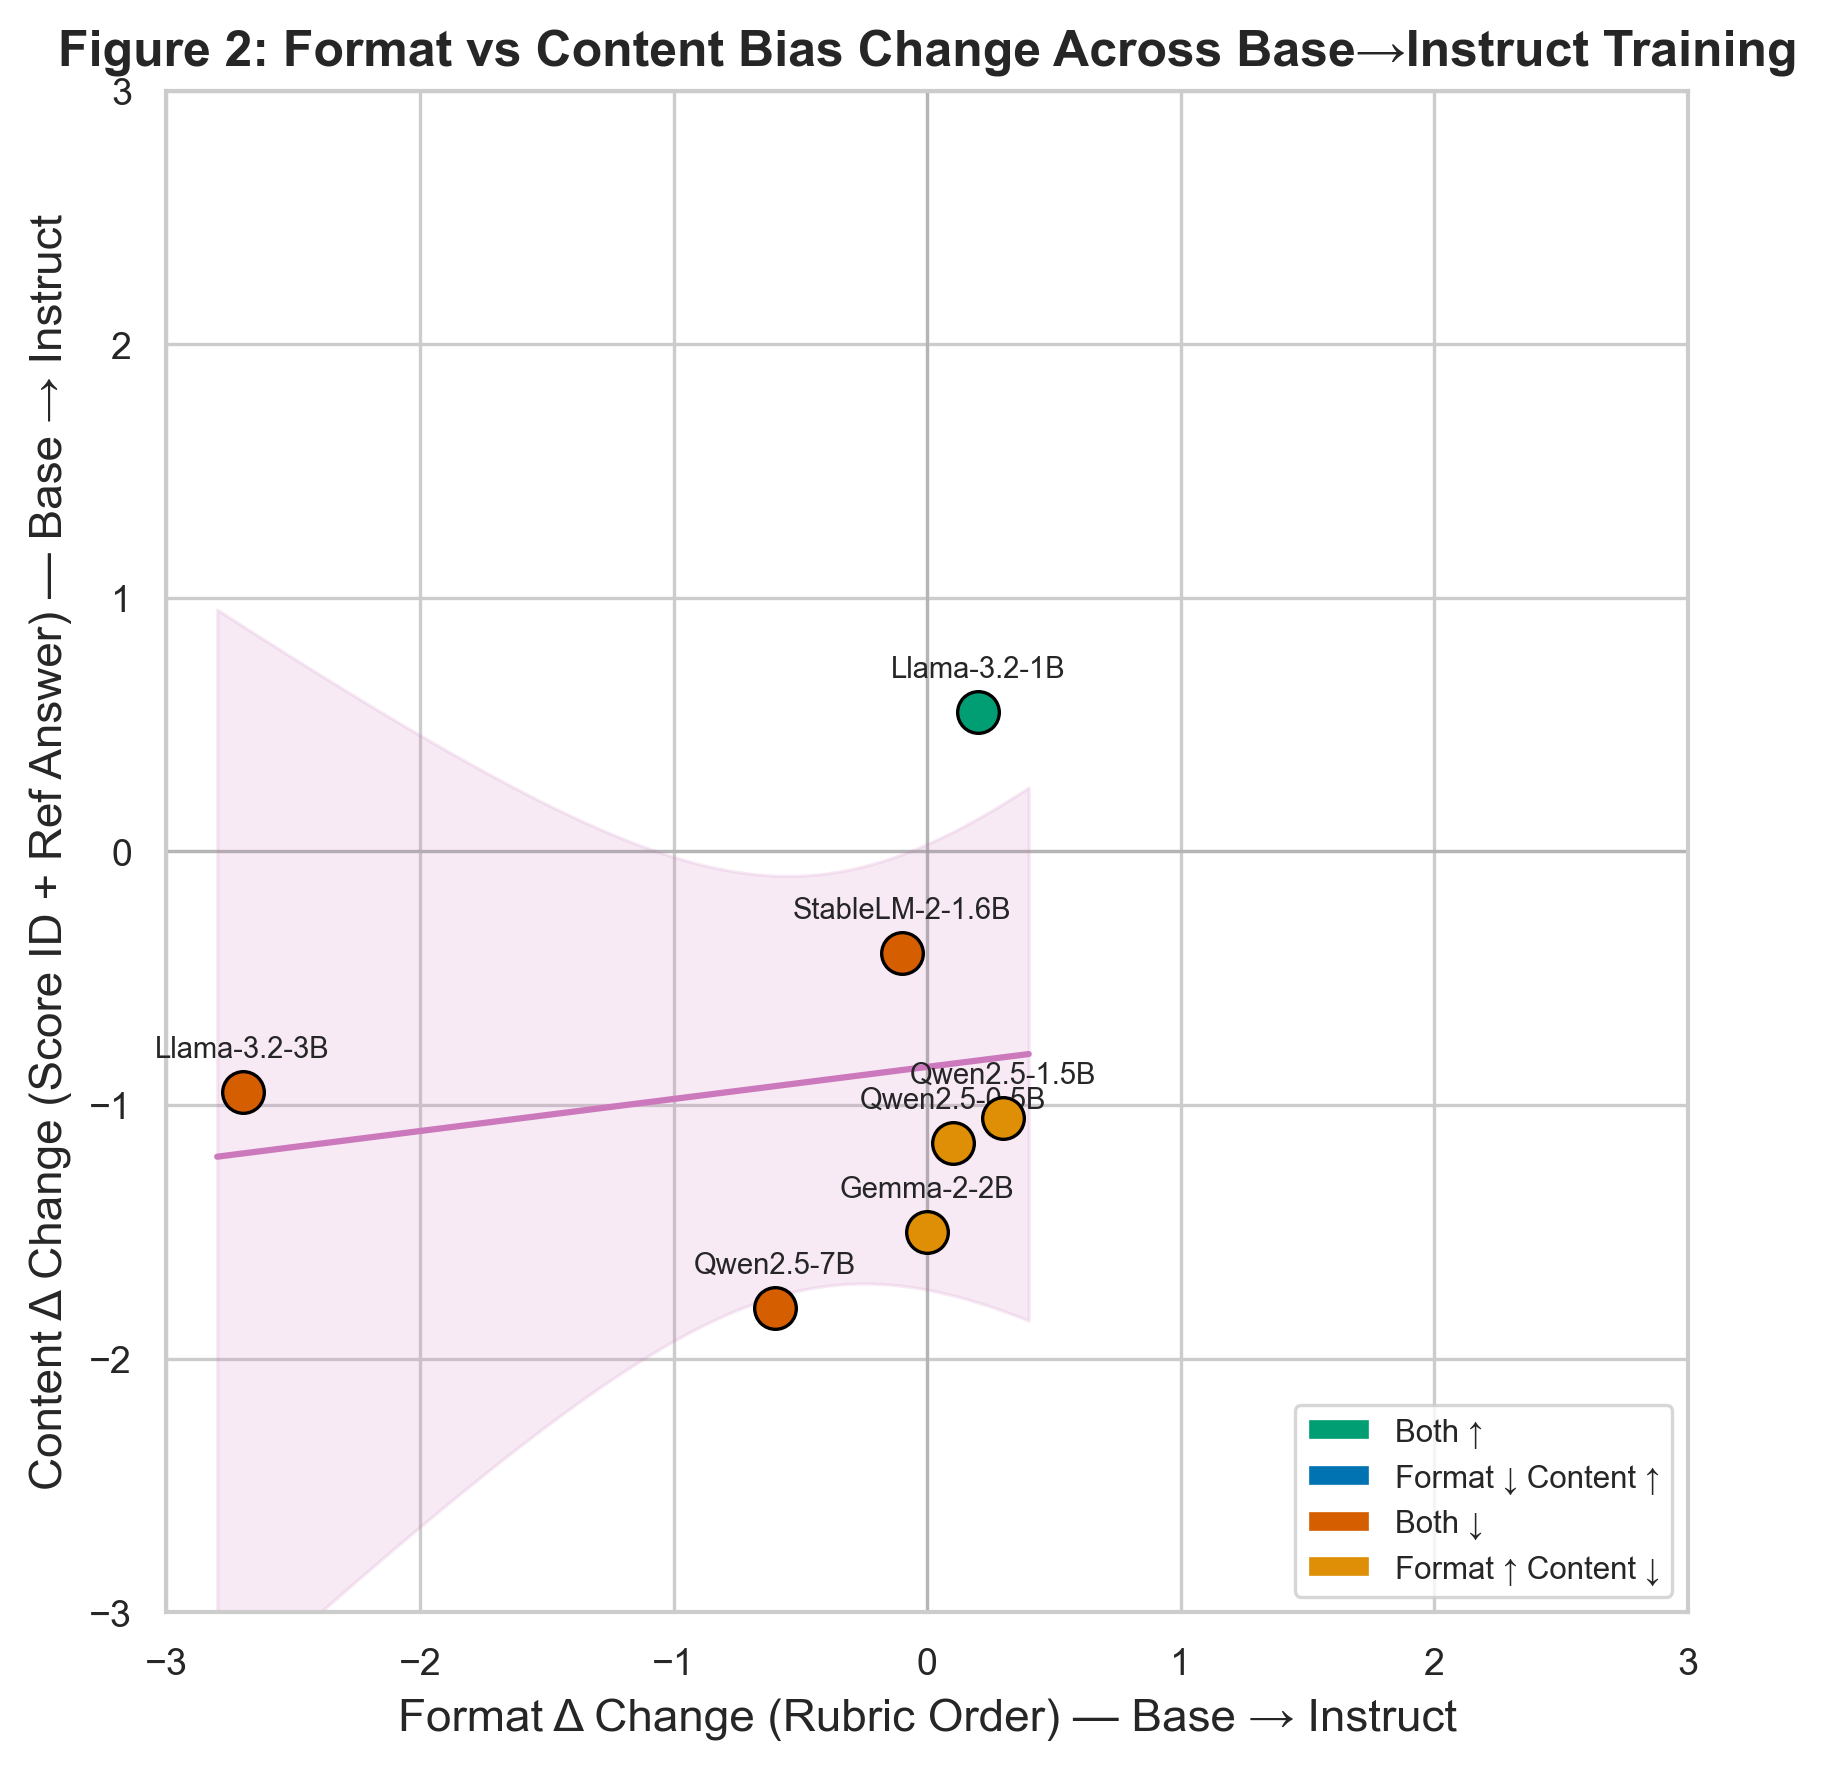
\includegraphics[width=\textwidth]{figures/fig2_format_content_scatter.png}
\caption{Format $\Delta$ change vs content $\Delta$ change for 9 base-instruct families.}
\label{fig:format_content_scatter}
\end{figure}

\begin{figure}[h]
\centering
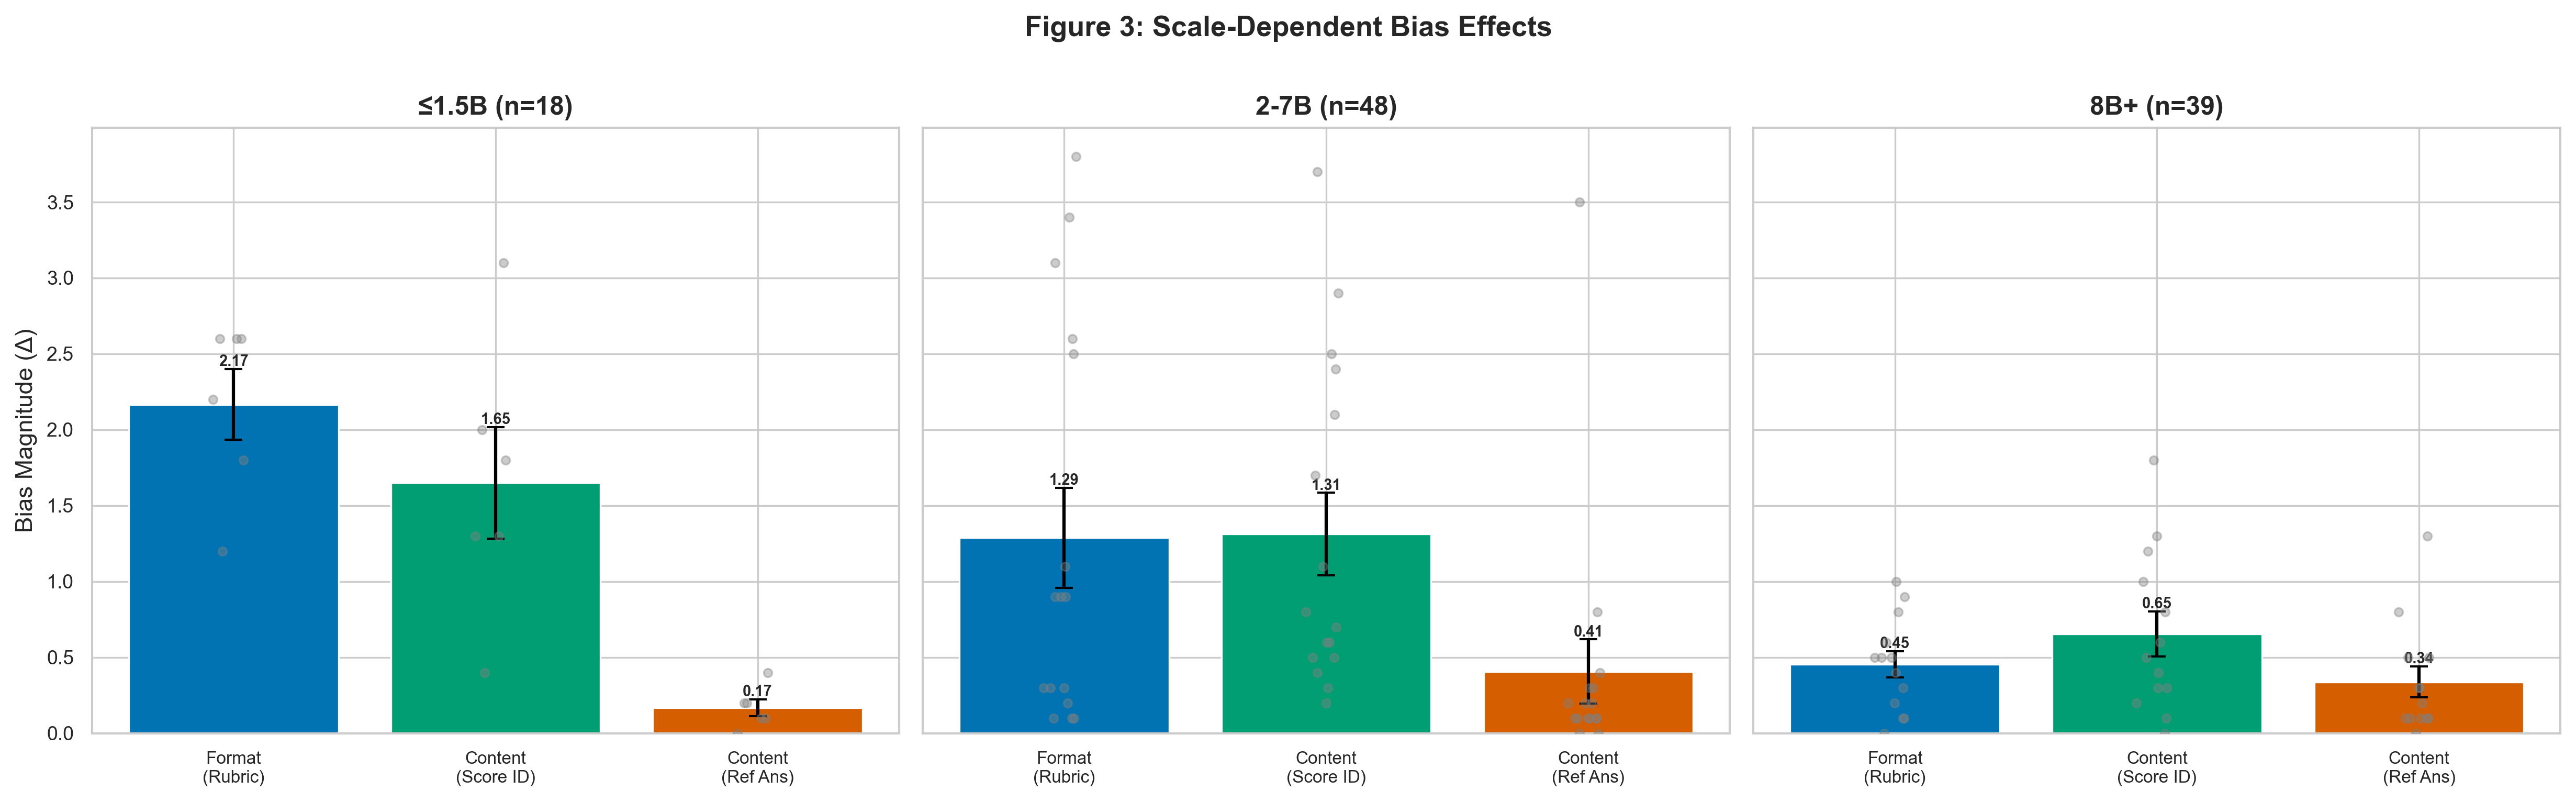
\includegraphics[width=\textwidth]{figures/fig3_scale_dependent.png}
\caption{Scale-dependent differential effect.}
\label{fig:scale_dependent}
\end{figure}

\subsection{Per-Model Bias Scores}

Table~\ref{tab:per_model} shows per-model bias scores. Score ID bias has the largest variance (range $0.00$--$1.80$).

\begin{table*}[h]
\centering\small
\caption{Per-model bias scores ($\Delta$) across 22 instruct models.}
\label{tab:per_model}
\begin{tabular}{lccc}
\toprule
\textbf{Model} & \textbf{Rubric} & \textbf{Score ID} & \textbf{Ref Ans} \\
\midrule
Command-R & 0.30 & 1.10 & 0.90 \\
DeepSeek-V3 & 0.20 & 0.80 & 0.30 \\
DeepSeek-V4-Flash & 0.30 & 0.50 & 0.30 \\
GLM-4.7 & 0.10 & 0.20 & 0.30 \\
GPT-OSS-20B & 0.10 & 0.10 & 0.10 \\
Gemini-2.5-Flash & 0.30 & 0.30 & 0.90 \\
Gemma3-12B & 0.90 & 0.30 & 0.90 \\
Gemma3-27B & 0.80 & 0.20 & 0.50 \\
Gemma3-4B & 0.20 & 0.50 & 0.10 \\
Hermes-3-70B & 0.80 & 1.80 & 0.50 \\
Hy3-295B & 1.00 & 1.20 & 0.60 \\
Llama-3.1-8B & 0.60 & 0.60 & 0.80 \\
Llama-3.2-3B & 0.40 & 0.60 & 0.20 \\
Lunaris-8B & 0.40 & 0.40 & 1.00 \\
Mistral-3.2-24B & 0.30 & 0.30 & 0.40 \\
Mistral-Nemo-12B & 0.30 & 1.00 & 0.50 \\
MythoMax-13B & 1.50 & 1.30 & 0.20 \\
Phi-4 & 0.60 & 0.70 & 0.10 \\
Qwen2.5-72B & 1.30 & 0.80 & 0.30 \\
Qwen2.5-7B & 0.70 & 1.70 & 0.10 \\
Qwen3-14B & 0.10 & 0.00 & 0.10 \\
Qwen3-8B & 1.20 & 0.50 & 0.00 \\
\midrule
\textbf{Mean} & \textbf{0.56} & \textbf{0.68} & \textbf{0.41} \\
\textbf{Std Dev} & \textbf{0.41} & \textbf{0.49} & \textbf{0.31} \\
\bottomrule
\end{tabular}
\end{table*}

\begin{figure*}[t]
\centering
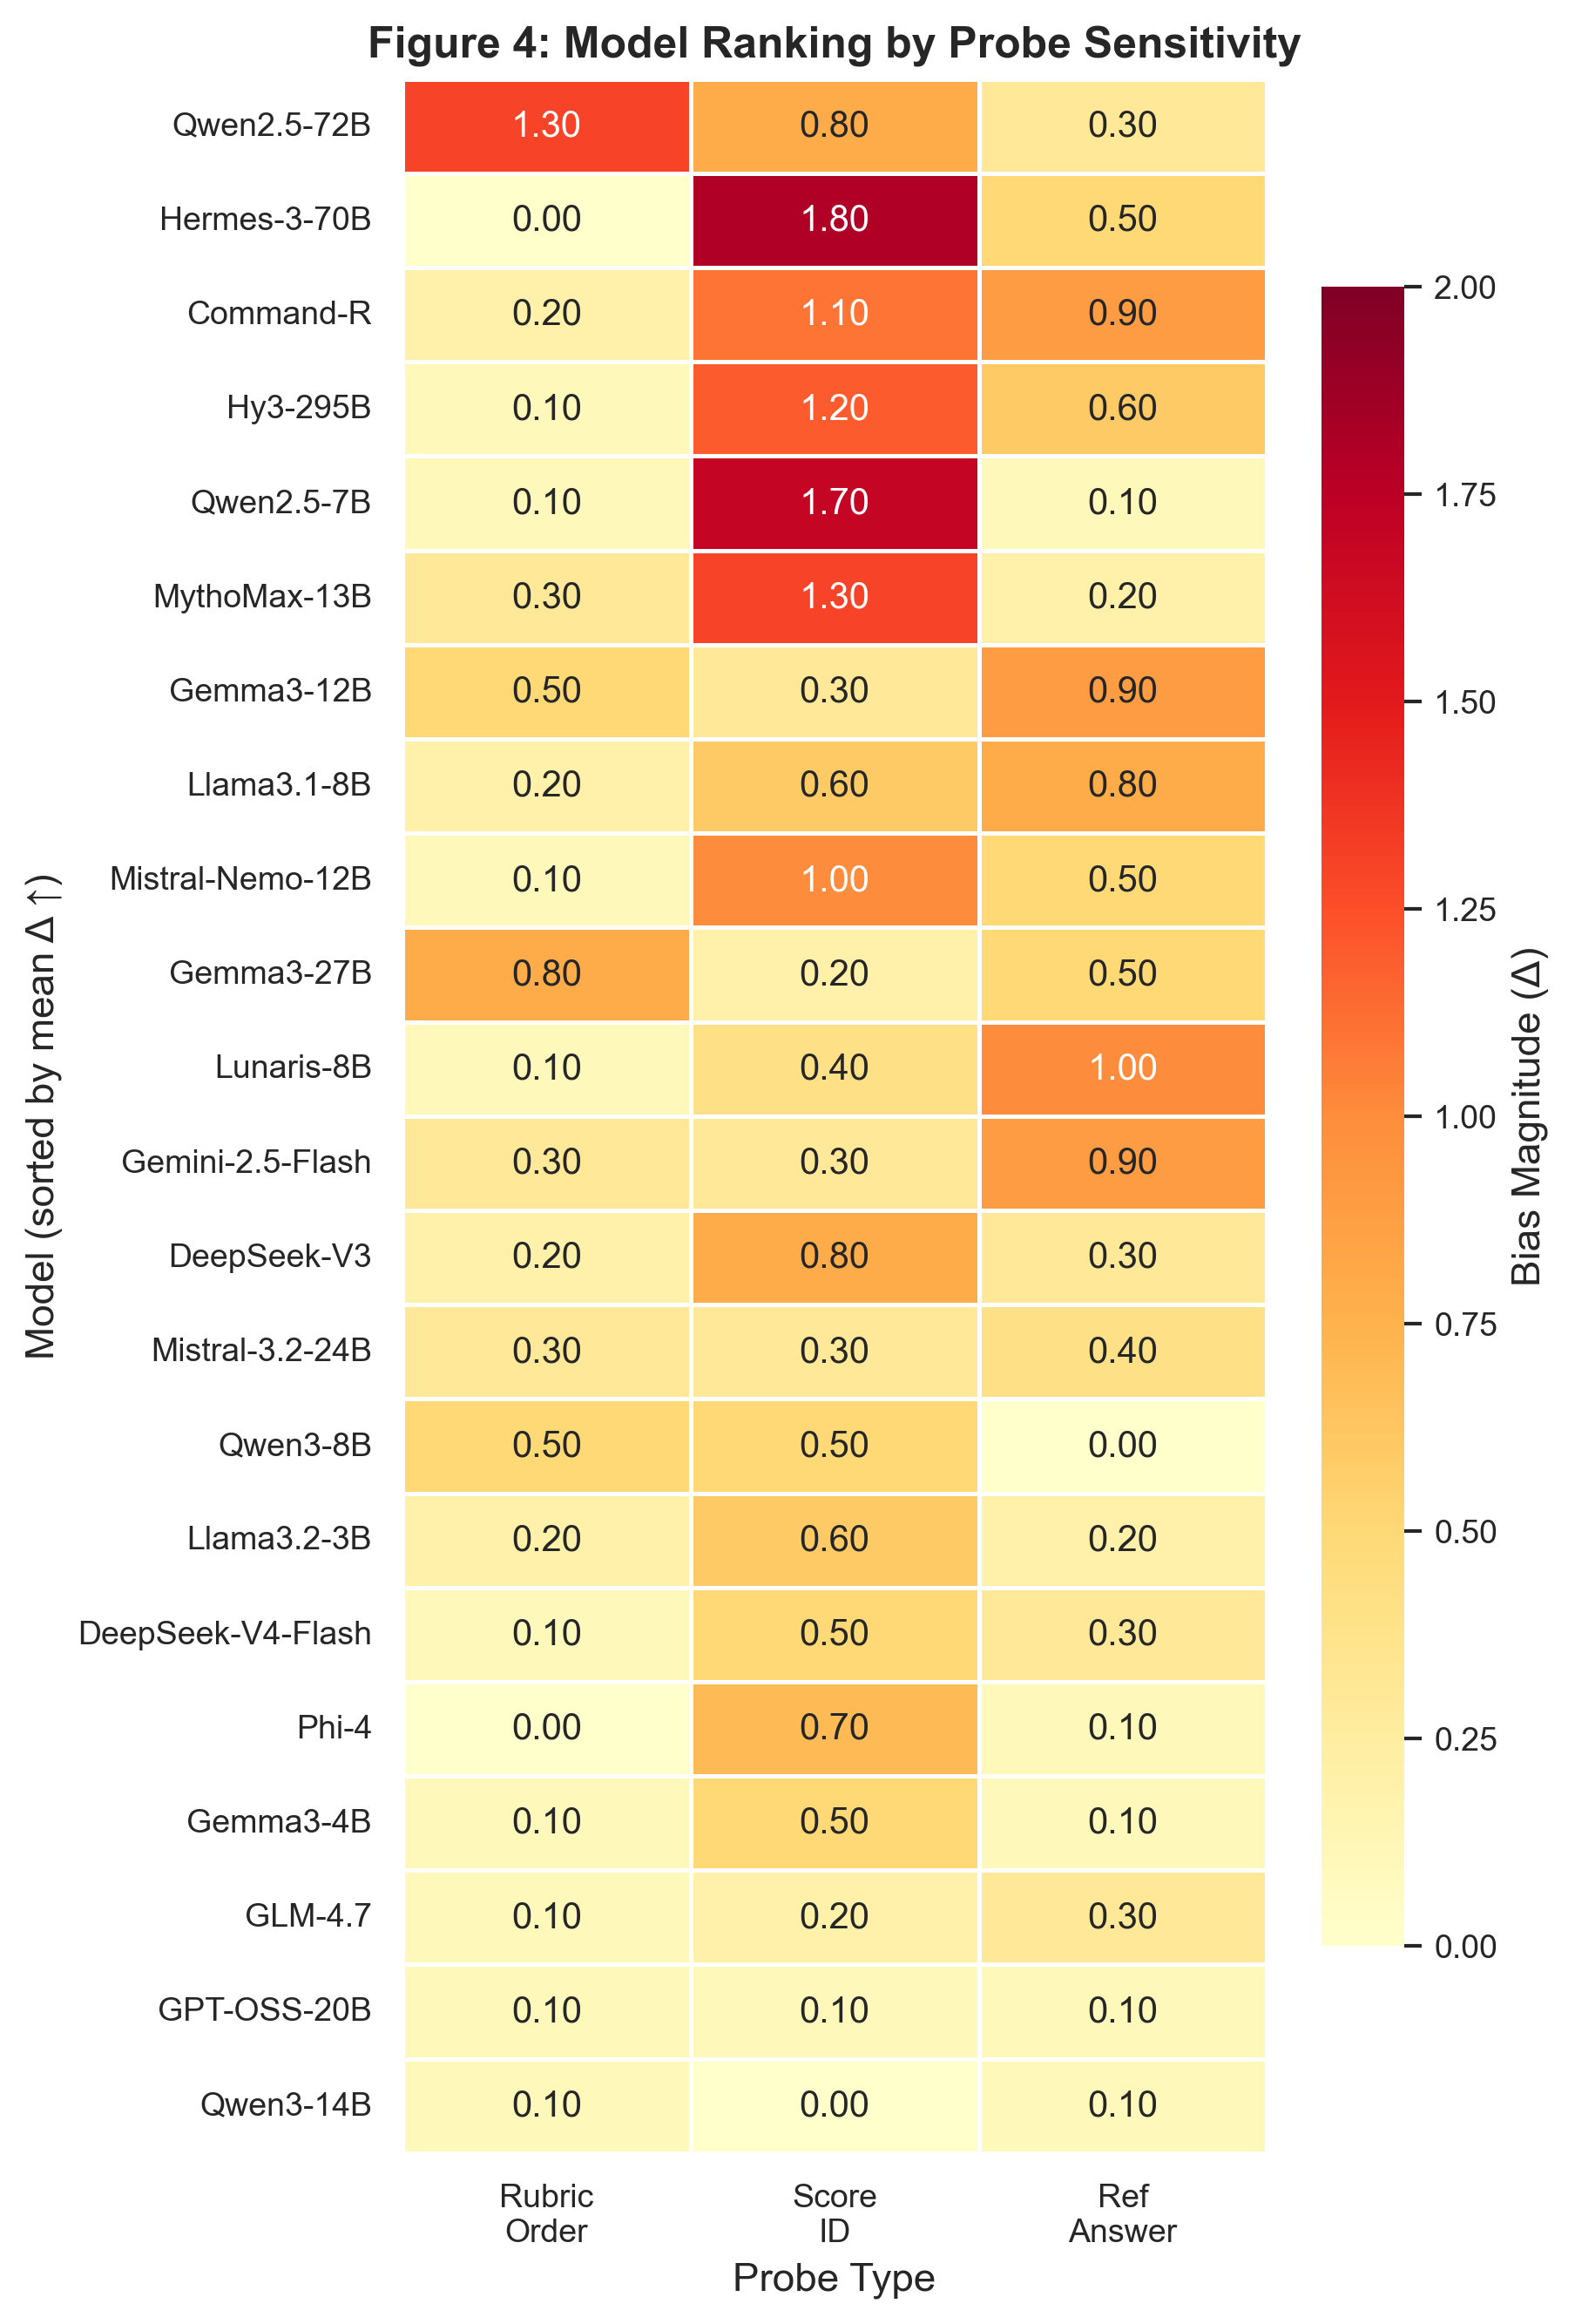
\includegraphics[width=\textwidth]{figures/fig4_model_ranking_heatmap.png}
\caption{Model ranking heatmap.}
\label{fig:model_ranking}
\end{figure*}

\subsection{Per-Family Analysis and Mitigation}
The seven RLHF families show the differential effect (format decrease, content increase). SFT+DPO (Mistral 7B) and SFT-only (StableLM 2) families show different patterns. The differential effect suggests bias mitigation must address two separate channels: format robustness and content sensitivity.

\subsection{Alternative Explanations}
We examine four alternatives: (1) global scoring shift---not supported (directions diverge); (2) single-family dominance---not supported; (3) probe ordering---identical for control and biased; (4) parser artifacts---numeric and letter variants independently show the same pattern. All four are inconsistent with the observed data.

\subsection{Statistical Analysis}
With N=9 families, paired $t$-tests show large effect sizes (Cohen's $d$ 1.20--2.38) but do not reach $p<0.05$. Bayesian analysis confirms scoring bias across the 22-model landscape ($\text{BF}_{10} > 10{,}000$). For the 7 T4 families, Score ID shows $\text{BF}_{10} = 298$ for base models (strong evidence bias exists).

\begin{figure}[h]
\centering
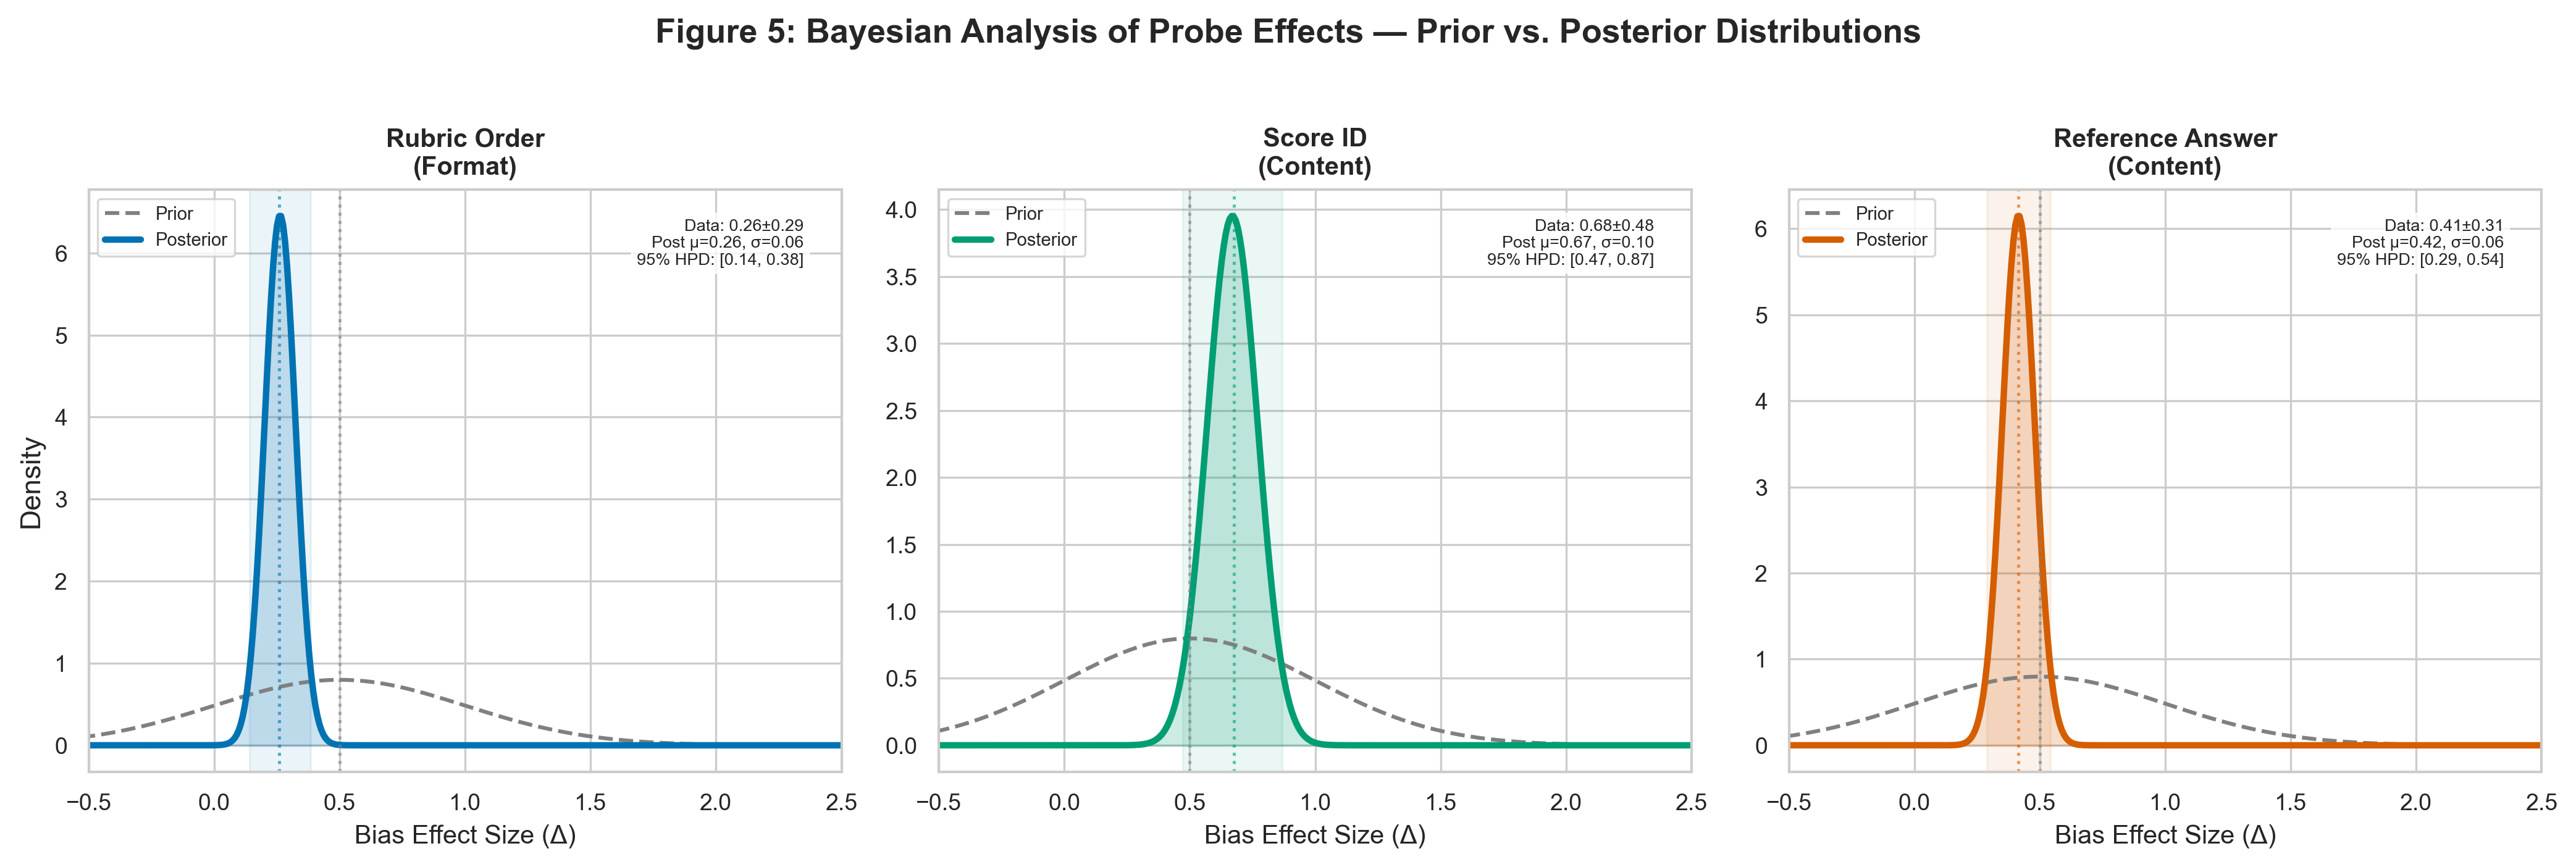
\includegraphics[width=\textwidth]{figures/fig5_bayesian_posteriors.png}
\caption{Bayesian posterior distributions.}
\label{fig:bayesian_posteriors}
\end{figure}

% ── DISCUSSION ──
\section{Discussion}

\paragraph{The differential effect.}
We propose the \textbf{Instruction-Induced Attention Redistribution (IIAR)} hypothesis: instruction tuning increases attention to all prompt features. However, per-layer attention-weight analysis does not support IIAR.

\begin{itemize}
    \item \textbf{0.5B:} Format $\kappa_f = 1.003$, Content $\kappa_c = 0.870$.
    \item \textbf{3B:} Format $\kappa_f = 0.879$, Content $\kappa_c = 1.035$.
\end{itemize}

\paragraph{Alternative: Format Efficiency Hypothesis.} Instruction tuning makes format parsing more efficient, with format attention decreasing from $23.7\%$ to $20.8\%$ at 3B. Content attention remains essentially unchanged ($1.06\% \to 1.09\%$). This suggests the content bias increase in larger models stems from increased helpfulness making models more susceptible to exemplar priming.

\paragraph{Implications.} Bias mitigation must address format robustness (naturally improved) and content sensitivity (worsened) as separate channels.

% ── LIMITATIONS ──
\section{Limitations}

We identify six limitations:
\begin{enumerate}
    \item \textbf{Item count (50).} Sufficient for observed effects ($d_{\min}=0.79$, observed $d=1.20$ to $2.38$).
    \item \textbf{9 families.} Format bias reduction consistent; content finding scale-dependent.
    \item \textbf{Descriptive parser.} Affects 11.1\% of one comparison; numeric and letter variants independently confirm findings.
    \item \textbf{English-only.} Generalizability to multilingual settings bounded.
    \item \textbf{Single prompt template.} Direction consistent, magnitude may vary.
    \item \textbf{No human baseline.} All claims are relative (base vs instruct).
\end{enumerate}

% ── BROADER IMPACT ──
\section{Broader Impact}

\paragraph{Ethics statement.}
This research was conducted in accordance with the NeurIPS Code of Ethics. No human subjects were involved. All models are publicly available. Total compute cost under \$3.

Our findings have three actionable implications. \textbf{For practitioners}: test multiple scoring formats, use both good and poor exemplars, report separate format and content bias scores. \textbf{For model developers}: improving format parsing during instruction tuning is achievable without increasing content susceptibility. \textbf{For benchmark designers}: use numeric labels by default.

% ── CONCLUSION ──
\section{Conclusion}

We investigated whether scoring bias originates from pre-training or instruction tuning. Across 31 model variants (54,000 judgments), we find instruction tuning has a differential effect: format-related bias decreases while content-related bias shows a scale-dependent increase in larger RLHF models. The 22-model landscape reveals Score ID bias as the largest concern ($\Delta=0.68$). Bayesian analysis confirms strong evidence for scoring bias across all probes. Our findings show scoring bias is modulated by instruction tuning---not inherent to pre-training---meaning mitigation strategies should target the alignment stage.

The \textbf{Format Efficiency Hypothesis}, supported by attention-weight evidence (format attention $23.7\%\to20.8\%$), provides a more parsimonious explanation than IIAR for the differential effect. All code and data are publicly available at \url{https://github.com/ssamba1/Scoring-Bias-in-LLM-as-a-Judge} and archived at \href{https://doi.org/10.5281/zenodo.21361920}{10.5281/zenodo.21361920}.

% ── Author Contributions ──
\section*{Author Contributions}
CRediT taxonomy: Conceptualization (lead), Methodology (lead), Software (lead), Validation (lead), Formal Analysis (lead), Investigation (lead), Data Curation (lead), Writing --- Original Draft (lead), Writing --- Review \& Editing (lead), Visualization (lead).

% ── Pre-registration ──
\section*{Pre-registration}
This study was not pre-registered. Research questions (RQ1--RQ4) and hypotheses (H1--H4) were specified before data analysis. Post-hoc analyses are explicitly noted.

% ── Acknowledgments ──
\section*{Acknowledgments}
We thank our research mentor for guidance and feedback. AI tools were used to assist in code generation and initial drafting. All experimental design, analysis, interpretation, and editing were performed by the author.

% ── Data Availability ──
\section*{Data Availability}
All code and data at \url{https://github.com/ssamba1/Scoring-Bias-in-LLM-as-a-Judge}. Frozen snapshot at \href{https://doi.org/10.5281/zenodo.21361920}{10.5281/zenodo.21361920}.

\bibliographystyle{unsrt}
\bibliography{references}

% ── Appendices ──
\appendix
\section{Model Details}
\label{app:models}
Full model cards are in \texttt{data/model\_cards/all\_models.md} and the repository.

\section{Full Results}
\label{app:results}
Per-model bias scores and item-level analysis are at \url{https://github.com/ssamba1/Scoring-Bias-in-LLM-as-a-Judge}.

\section{Formal Proofs}
\label{app:proofs}
The IIAR monotonicity theorem, differential direction corollary, and scaling law prediction are proved in the supplementary formal document.

\section{Reproducibility Instructions}
\label{app:reproduce}
Complete pipeline in \texttt{run\_all.sh}. Docker: \texttt{docker build -t scoring-bias . \&\& docker run scoring-bias}.

\end{document}
